%!TEX root = draft.tex
\section{Stacks With Fixed Pop Commit Points}\label{sec:stacks}

While the abstract queue implementation in Section~\ref{sec:queues} can be adapted to stacks~\footnote{The only modification is that the linearization point of a pop $lin(pop,d,k)$ with $d\neq{\tt EMPTY}$ is enabled only if $k$ is added by a push which is maximal in the happens-before order stored in the state.}, it can not simulate (through forward simulations) existing stack implementations like the Time-stamped Stack~\cite{DBLP:conf/popl/DoddsHK15} where the linearization points of the pop operations are not fixed. In this section, we define an abstract implementation which simulates such implementations provided that the point in time where the return value of a pop operation is determined corresponds to a fixed action. To demonstrate the use of this abstract implementation we provide a correctness proof for a simplified version of Time-Stamped Stack that preserves its most complex behaviors.

\subsection{Abstract stack implementation}


\begin{wrapfigure}{l}{5.4cm}
\vspace{-11mm}
\begin{lstlisting}
struct Node{
  int data;
  int ts;
  Node* next;
  boolean taken;
};
Node* pools[maxThreads];
int TS = 0;   

void push(int x) {
  Node* n = new Node(x,MAX_INT,
                        null,false);
  n->next = pools[myTID];
  pools[myTID] = n;
  int i = TS++;
  n->ts = i;
}
int pop() {
 boolean success = false;
 int maxTS = -1;
 Node* youngest = null;
 while ( !success ) {
   maxTS = -1; youngest = null;
   for(int i=0; i<maxThreads; i++){
     Node* n = pools[i];
     while (n->taken && n->next != n)
       n = n->next;
     if(maxTS < n->ts) {
       maxTS = n->ts; youngest = n;
     }
   }
   if (youngest != null)
     success=CAS(youngest->taken,
                       false,true);
 }
 return youngest->data;
}
\end{lstlisting}
\vspace{-6mm}
\caption{Time-Stamped Stack. We assume that every statement is atomic.}
\label{fig:TimeStamped}
\vspace{-1mm}
\end{wrapfigure}
We explain the meaning of the commit points on a simplified version of the Time-Stamped Stack~\cite{DBLP:conf/popl/DoddsHK15} given in Figure~\ref{fig:TimeStamped}. This stack implementation maintains a vector of singly-linked lists, one for each thread, where list nodes contain a data value (field {\tt data}), a timestamp (field {\tt ts}), the next pointer (field {\tt next}), and a boolean flag indicating whether the node represents a value removed from the stack (field {\tt taken}). Initially, each list contains a sentinel dummy node pointing to itself with timestamp $-1$ and the flag {\tt taken} set to {\tt false}.

Pushing a value to the stack proceeds in several steps: adding a node with maximal timestamp in the list associated to the thread executing the push (given by the special variable {\tt myTID}), asking for a new timestamp (given by the value of the shared integer {\tt TS}), and updating the timestamp of the added node. Popping a value from the stack consists in traversing all the lists, finding the first element which doesn't represent a removed value (i.e., {\tt taken} is {\tt false}) in each list, and selecting the element with the maximal timestamp. A compare-and-swap (CAS) is used to set the {\tt taken} flag of this element to {\tt true}. The procedure restarts if the CAS fails.

\begin{figure}[t]
\centering
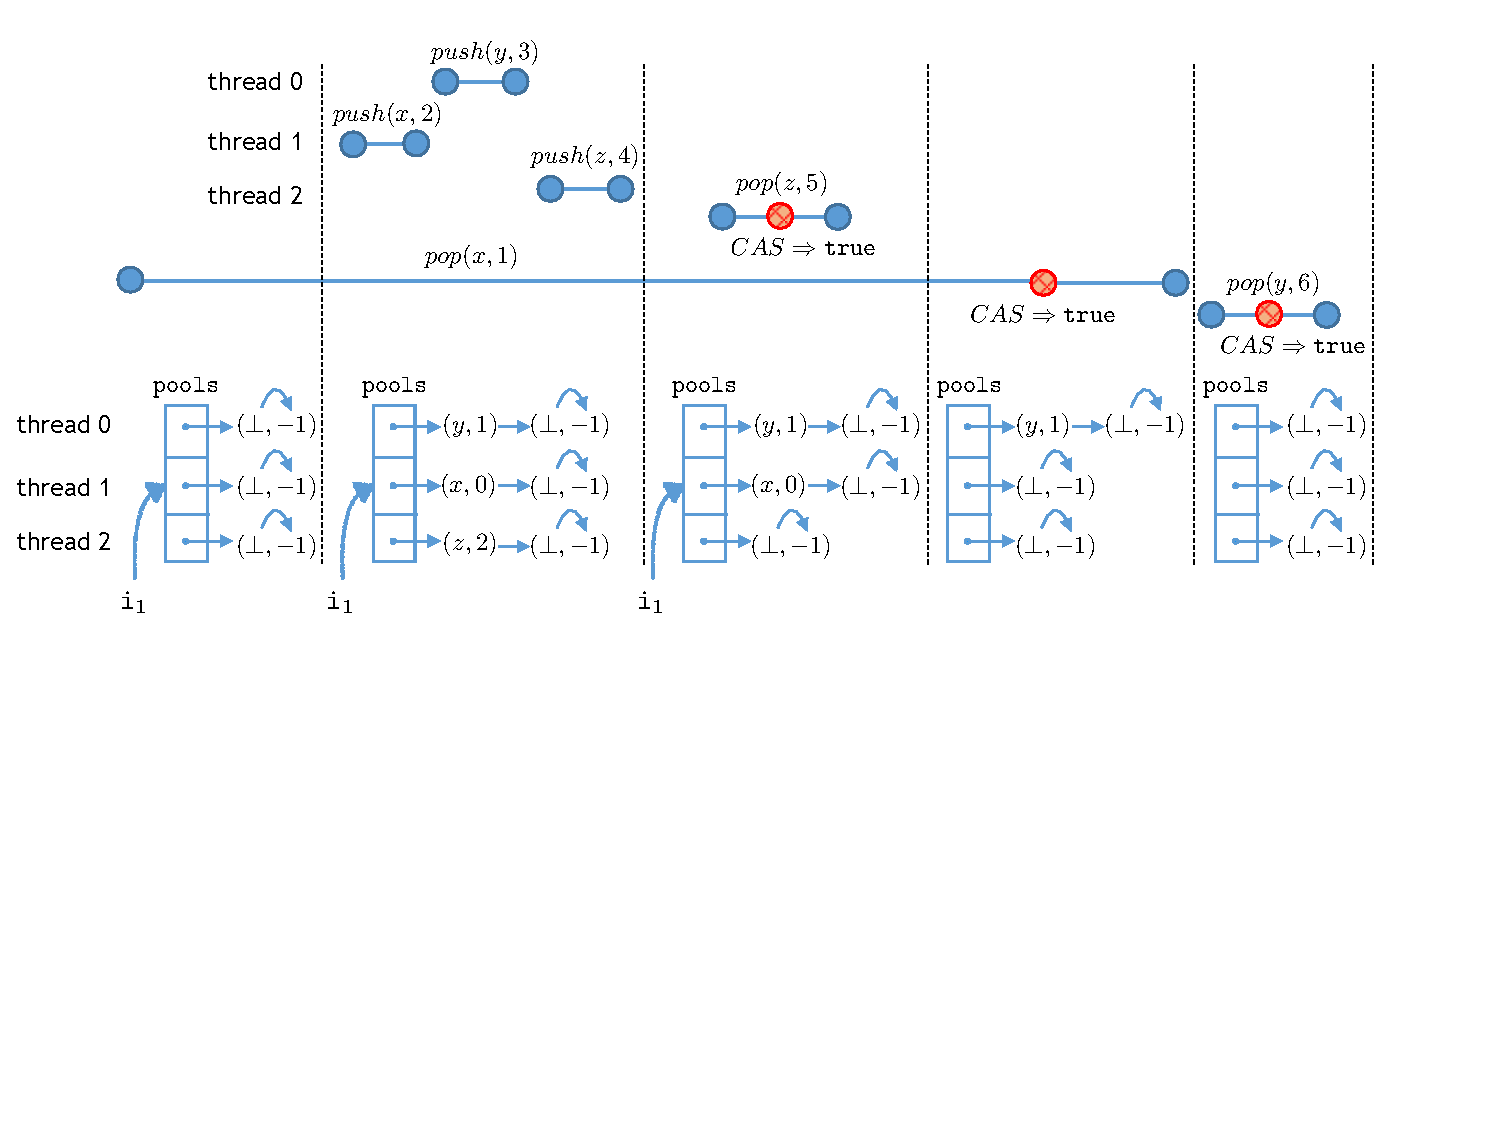
\includegraphics[width=11cm]{fig-timeStamp.pdf}
\caption{An execution of the Time-Stamped Stack. An operation is pictured by a line delimited by two circles denoting the call and respectively, the return action. For pop operations, we introduce another circle to represent a CAS returning {\tt true} which is the commit point of that operation. The state of the library after an execution prefix delimited at the right by a dotted line is pictured in the bottom part (the picture immediately to the left of the dotted line). Also, ${\tt i}_1$ denotes the value of {\tt i} in the pop operation with identifier 1.}
\label{fig:commit}
\end{figure}


The push operations don't have a fixed linearization point because adding a node to a list and updating its timestamp are not executed in a single atomic step. The nodes can be added in an order which is not consistent with the order between the timestamps assigned later in the execution. Also, the value added by a push that just added an element to a list can be popped before the value added by a completed push (since it has a maximal timestamp). The same holds for pop operations. The only reasonable choice for a linearization point is a successful CAS (that results in updating the field {\tt taken}).

TODO GIVE AN EXAMPLE TO SHOW THE ISSUE WITH POP LINEARIZATION POINTS, AND TO SHOW THAT COMMIT POINTS ARE RIGHT LIMITS FOR THE INTERVAL OF A LIN POINT, I.E., A POP WITH A LATER COMMIT POINT CAN BE LINEARIZED BEFORE. NEED ONLY 2 POPS IN AN EXECUTION 

We consider a set of actions $Com(pop)=\set{com(pop,d,k):d\in\<Vals>, k\in\<Ops>}$, called \emph{commit points}, representing actions of a pop operation where its return value is determined. Usually, a stack implementation stores the pushed values into a data structure, e.g., a singly-linked list, and a pop operation contains an action (typically, a compare-and-swap) that removes an element from this data structure (or sets a flag associated to this element to a ``deleted'' state). Such an action represents a commit point since the pop operation will return the value stored in this element. 

// Initially each pool[i] points to a 
// sentinel dummy node with ts = -1, 
// next = null, taken=false


TODO DESCRIBE THE TIME-STAMPED STACK, EXPLAIN THAT NO METHOD HAS A FIXED LIN POINT, GIVE THE COMMIT POINTS, SHOW THAT COMMIT POINTS ARE NOT LIN POINTS

COMMIT POINTS ARE LINEARIZATION POINTS WHEN THE LIBRARY IS INTERPRETED AS A MULTISET

We define an abstract stack implementation $AbsS$ over alphabet $C\cup R\cup Com(pop)$ that essentially, similarly to $AbsQ$, maintains the happens-before order of the push operations whose value has not been yet removed. However, since the commit points are not necessarily linearization points, the pop operations are treated differently. Intuitively, each pop operation starts by taking a snapshot of the completed push operations which are maximal in the happens-before order and continuously tracks the push operations which are overlapping with it. The commit point is enabled only if the return value corresponds to one of the push operations in the initial snapshot, or to a push happening earlier when the values from the initial snapshot are removed by other pop operations, or to one of the push operations that overlaps with the pop. TODO EMPTY

\begin{wrapfigure}{l}{7cm}
\vspace{-8mm}
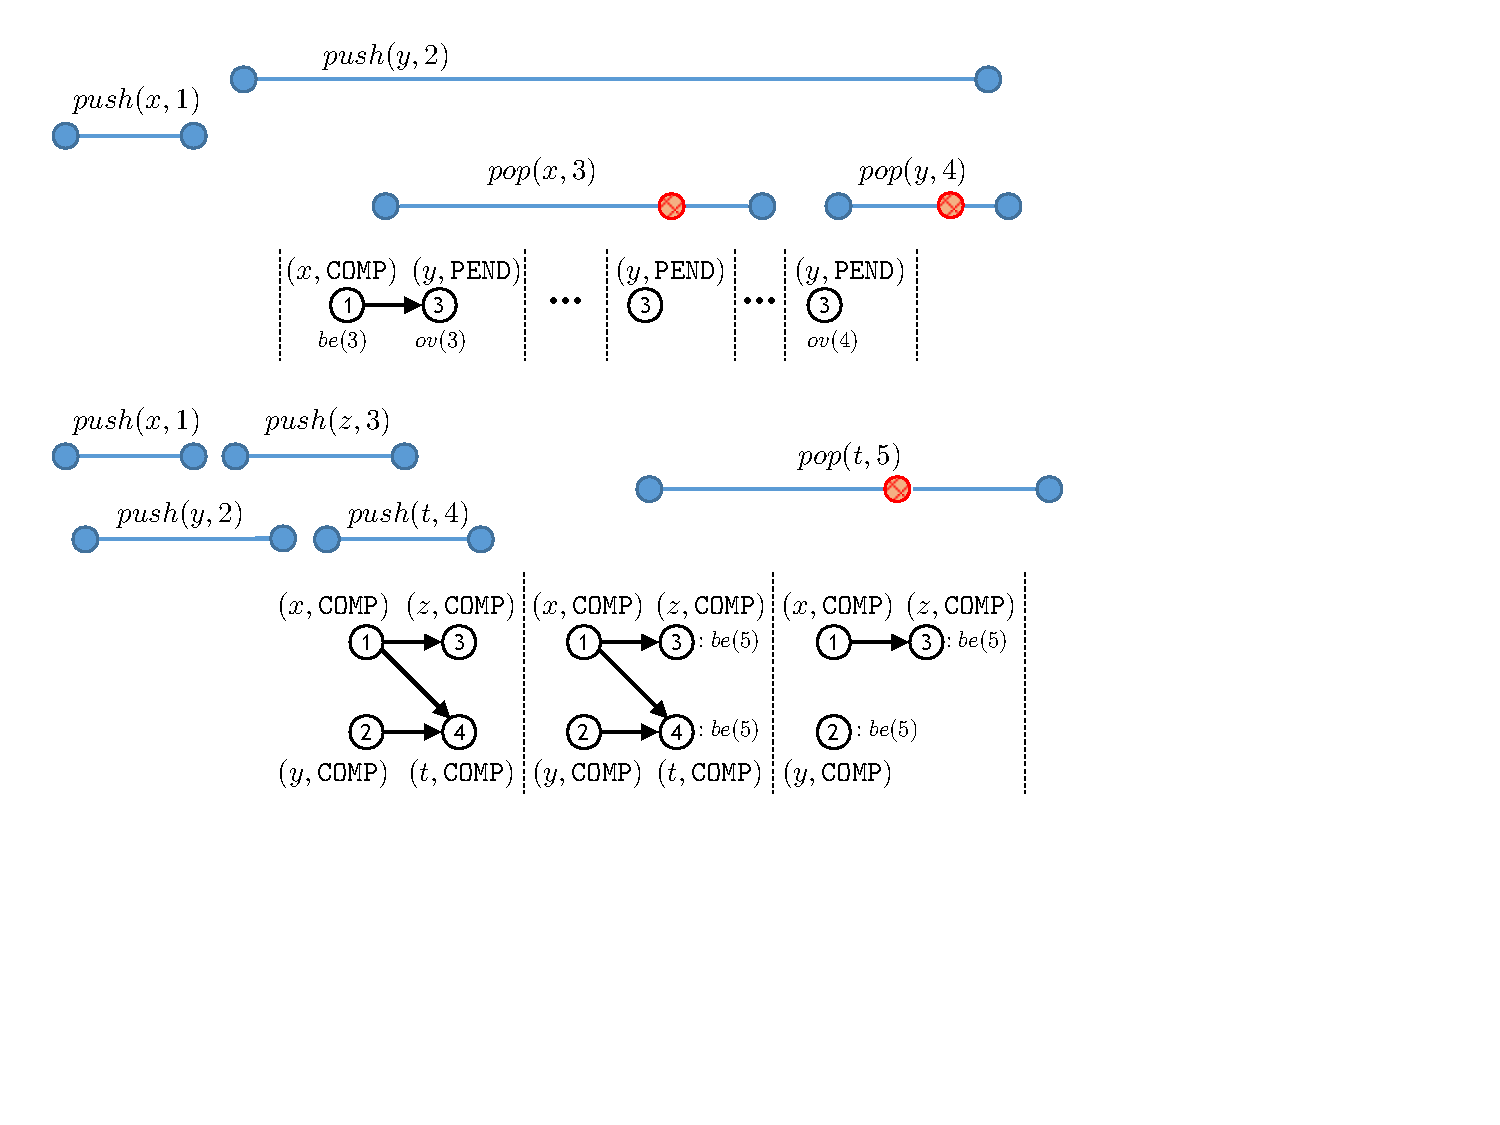
\includegraphics[width=7cm]{fig-stack.pdf}
%
%\vspace{2mm}
%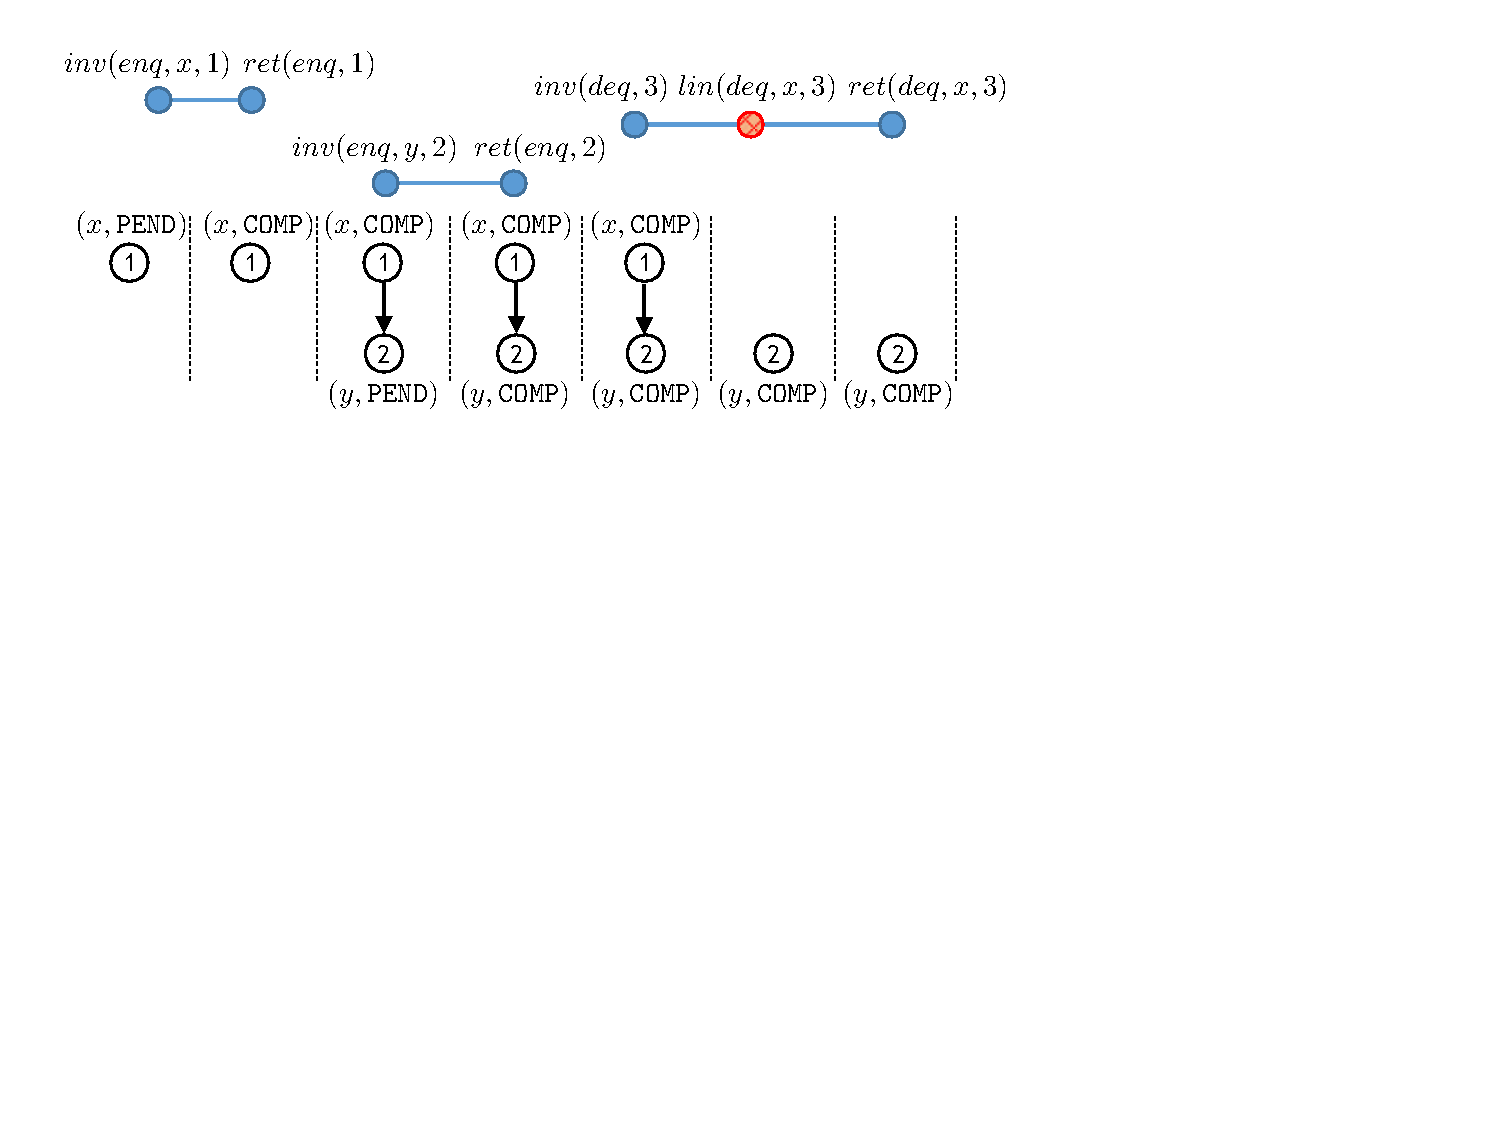
\includegraphics[width=7cm]{fig-queue2.pdf}
\vspace{-5mm}
\caption{Simulating stack histories with $AbsS$.}
\label{fig:stackSim}
\vspace{-6mm}
\end{wrapfigure}
Figure~\ref{fig:stackSim} pictures two executions of $AbsQ$ for two extended histories (that include dequeue linearization points). The state of $AbsQ$ after each action is pictured as a graph below the action. The nodes of this graph represent enqueue operations and the edges happens-before constraints. Each node is labeled by a value (the input of the enqueue) and a flag {\tt PEND} or {\tt COMP} showing whether the operation is pending or completed. For instance, in the case of the first history, the dequeue linearization point $lin(deq,y,3)$ is enabled because the current happens-before contains a \emph{minimal} enqueue operation with input $y$. Note that a linearization point $lin(deq,x,3)$ is also enabled at this state.


TODO AN EXAMPLE FOR EACH CASE (HISTORIES OF THE TIME-STAMPED STACK)



The states of $AbsS$ are tuples $\tup{O,<,\ell,rv,cp,be,ov}$ where $O\subseteq \<Ops>$ represents a set of operation identifiers (of previously invoked push operations), $<\subseteq O\times O$ is a strict partial order over $O$, $\ell: O -> \<Vals>\times\{\tt{PEND,\tt{COMP}}\}$ labels every identifier in $O$ with a value and a flag that records whether the operation is pending or completed, $be:\<Ops> ~> 2^O$ records push operations that were maximal before a pop started or happening earlier provided that the values of all the push happening later have been removed, and $ov: \<Ops> ~> 2^O$ records push operations overlapping with a pop.
The initial state has all these components set to $\emptyset$ and the transition relation $->$ is defined in Figure~\ref{fig:transitions:AbsS}.

\begin{figure} [t]
{\scriptsize
  \centering
  \begin{mathpar}
    \inferrule[call-push]{
      k\not\in dom(cp) \\ 
      d\neq {\tt EMPTY}
    }{
      O,<,\ell,rv,cp,be,ov 
      \xrightarrow{inv(push,d,k)} \\
      O\cup\{k\},<\cup\ {\tt COMP}(O)\times\{k\},\ell[k\mapsto (d,{\tt PEND})],rv,cp[k\mapsto 1],be,ov[\forall k'.\ k'\mapsto ov(k')\cup \{k\}]
    }\hspace{5mm}

    \inferrule[call-pop]{
      k\not\in dom(cp) \\
    }{
      O,<,\ell,rv,cp,be,ov
      \xrightarrow{inv(pop,k)} \\
      O,<,\ell,rv,cp[k\mapsto 1],be[k\mapsto maxCo(O)],ov[k\mapsto {\tt PEND}(O)]
    }\hspace{5mm}
    
    \inferrule[ret-pop]{
       cp(k) = 2 \\
       rv(k)=d  
    }{
      O,<,\ell,rv,cp,be,ov
      \xrightarrow{ret(pop,d,k)}
      O,<,\ell,rv,cp[k\mapsto 3],be,ov
    }\hspace{5mm}

    \inferrule[ret-push1]{
      cp(k) = 1 \\
      k \in O \\
      \ell(k) = (d,{\tt PEND}) 
    }{
      O,<,\ell,rv,cp,be,ov
      \xrightarrow{ret(push,k)}
      O,<,\ell[k\mapsto (d,{\tt COMP})],rv,cp[k\mapsto 2],be,ov
    }\hspace{5mm}
    
    \inferrule[ret-push2]{
      cp(k) = 1 \\
      k \not\in O 
    }{
      O,<,\ell,rv,cp,be,ov
      \xrightarrow{ret(push,k)}
      O,<,\ell,rv,cp[k\mapsto 2],be,ov
    }\hspace{5mm}

    \inferrule[lin-pop1]{
       cp(k) = 1 \\
       d\neq{\tt EMPTY} \\
       k'\in be(k)\cup ov(k)\land \ell_1(k')=d \\
       \forall k_1.\ k'\not\in be(k_1) \Rightarrow be'(k_1)=be(k_1) \\     \\
       \forall k_1.\ k'\in be(k_1) \Rightarrow be'(k_1)=(be(k_1)\setminus\{k'\})\cup \{k_2: k_2\in pred_{<}(k') \land \forall k_3. k_2<k_3 => k_3\not\in be(k_1)\} \\
    }{
      O,<,\ell,rv,cp,be,ov
      \xrightarrow{com(pop,d,k)} \\
      O\setminus \{k'\},<\uparrow k',\ell,rv[k\mapsto d],cp[k\mapsto 2],be',ov %be[\forall k''.\ k'\in be(k'') \Rightarrow k'' \mapsto (be(k'')\cup pred_{<}(k'))\setminus\{k'\}]
    }\hspace{5mm}

    \inferrule[lin-pop2]{
       cp(k) = 1 \\
       be(k)=\emptyset
    }{
      O,<,\ell,rv,cp,be,ov
      \xrightarrow{com(pop,{\tt EMPTY},k)}
      O,<,\ell,rv[k\mapsto {\tt EMPTY}],cp[k\mapsto 2],be,ov
    }\hspace{5mm}

    
      \end{mathpar}
  }
 \vspace{-5mm}
  \caption{The transition relation of $AbsQ$. We use the following notions: $f[\forall k.guard(k)=> k\mapsto expr(k)]$ is the function $g$ defined by $g(k)=f(k)$ for all $k$ such that $guard(k)$ is false, and $g(k)=expr(k)$ otherwise, $maxCo(O)$ is the set of maximally completed operations in $O$, i.e., $maxCo(O)=\set{k\in O: \ell_1(k)={\tt COMP}, \forall k'\in O.\ k' < k \vee \ell_1(k')={\tt PEND}}$, ${\tt PEND}(O)=\{k\in O: \ell_2(k)={\tt PEND}\}$, and $pred_{<}(k')$ is the set of immediate predecessors of $k'$ according to $<$, i.e., $pred_{<}(k')=\set{k\in O: k < k'\land \forall k''\in O.\ k'' > k' \vee k'' < k}$.%\textcolor{red}{call-push should have $d \neq EMPTY$ in the premise. If I understand correctly, there is a problem change in $be$ in lin-pop1 rule. What I understand is we move $k''$ to every predecesoor of $k'$. But we should not move it to predecessor of $k'$ if this predecessor has a successor $m$ such that $m \in be(k'')$. Is this case reflected in your definition. Please read sub-bullet 4 of bullet 4 in the definition of $L_I$ in my document. Lin-pop2 seems ok for me. Last note: Bibliography seems not correct to me.} 
  }
  \label{fig:transitions:AbsS}
\vspace{-6mm}
\end{figure}

Let $AbsS_0$ be the standard abstract implementation of a concurrent stack (where elements are stored in a sequence, a push operation adds atomically an element at the beginning of the sequence, and a pop operation removes atomically an element from the beginning of the sequence)~\footnote{For $\<Methods>=\{push,pop\}$, the alphabet of $AbsS_0$ is $C\cup R\cup Lin$.}.
The following result states that the library $AbsS$ has exactly the same set of histories as $AbsS_0$ (see Appendix~\ref{app:absImplStack} for a proof).

\begin{theorem}\label{th:absImplStack}
$AbsS$ is a refinement of $AbsS_0$ and vice-versa.
\end{theorem}

A trace of a queue implementation is called \emph{$Com(pop)$-complete} when every completed pop has a commit point, i.e., TODO. A stack implementation $L$ over alphabet $\Sigma$ is called \emph{with fixed pop commit points} if{f} $C\cup R\cup Com(pop)\subseteq \Sigma$ 
and every trace $@t\in Tr(L)$ is $Com(pop)$-complete.

TODO NEEDS DATA INDEPENDENCE FOR THE COMMIT POINT TRANSITIONS TO BE DETERMINISTIC

As a consequence of Theorem~\ref{th:forSim}, $C\cup R\cup Com(pop)$-forward simulations are a sound and complete proof method for showing the correctness of a stack implementation with fixed pop commit points (up to the correctness of the commit points). 

TODO EXPLAIN THAT THIS IS DIFFERENT W.R.T. QUEUES ($Abs_0$ doesn't have commit points).

\begin{corollary}
A stack implementation $L$ with fixed pop commit points is a $C\cup R\cup Com(pop)$-refinement of $AbsS$ if{f} there exists a $C\cup R\cup Com(pop)$-forward simulation from $L$ to $AbsS$.
\end{corollary}


\subsection{A Correctness Proof For Time-Stamped Stack}





